% \special{dvipdfmx:config z 0}
\documentclass[UTF8,a4paper,AutoFakeBold,AutoFakeSlant]{ctexart}
\usepackage[a4paper,left=2.8cm,right=2.6cm,top=3.7cm,bottom=3.5cm]{geometry}
% \usepackage{ctex}
% \usepackage{xeCJK}
\usepackage{graphicx}
\usepackage{pythonhighlight}
\usepackage[mathscr]{eucal}
\usepackage{mathrsfs}
\usepackage{booktabs}
\usepackage{capt-of} 
\usepackage{hyperref} 
\usepackage{abstract}
\usepackage{amsmath}
\usepackage{listings}
\usepackage{color}
\usepackage{caption}
\usepackage{subfigure}
\usepackage{enumerate}
\usepackage{amsfonts} 
\usepackage{CJK,CJKnumb}
\usepackage{float}
% \usepackage{gbt7714}
\usepackage{framed}
\usepackage{multirow}
\usepackage{animate}


\newcommand{\song}{\CJKfamily{song}}    % 宋体   (Windows自带simsun.ttf)
\newcommand{\fs}{\CJKfamily{fs}}        % 仿宋体 (Windows自带simfs.ttf)
\newcommand{\kai}{\CJKfamily{kai}}      % 楷体   (Windows自带simkai.ttf)
\newcommand{\hei}{\CJKfamily{hei}}      % 黑体   (Windows自带simhei.ttf)
\newcommand{\li}{\CJKfamily{li}}        % 隶书   (Windows自带simli.ttf) 
\newcommand{\ssong}{\CJKfamily{STSong}}

\xeCJKsetup{SlantFactor = 0.3}
% \xeCJKsetup{SlantFactor = -0.7}
\setCJKmainfont[BoldFont=SimHei, SlantedFont=KaiTi]{SimSun}



% -- 中文字体 --
%\setCJKmainfont{Microsoft YaHei}  % 微软雅黑
%\setCJKmainfont{YouYuan}  % 幼圆
%\setCJKmainfont{NSimSun}  % 新宋体
%\setCJKmainfont{KaiTi}    % 楷体
% \setCJKmainfont{SimSun}   % 宋体
%\setCJKmainfont{SimHei}   % 黑体
% \setCJKfamilyfont{hwsong}{STSong}
 
% -- 英文字体 --
% \setmainfont{Times New Roman}
% \setmainfont{DejaVu Sans}
% \setmainfont{Latin Modern Mono}
% \setmainfont{Consolas}
% \setmainfont{Courier New}


\usepackage{xcolor}  	%高亮使用的颜色
\definecolor{commentcolor}{RGB}{85,139,78}
\definecolor{stringcolor}{RGB}{206,145,108}
\definecolor{keywordcolor}{RGB}{34,34,250}
\definecolor{backcolor}{RGB}{220,220,220}

\usepackage{accsupp}	
\newcommand{\emptyaccsupp}[1]{\BeginAccSupp{ActualText={}}#1\EndAccSupp{}}

\usepackage{listings}
\lstset{						%高亮代码设置
	language=python, 					%Python语法高亮
	linewidth=0.95\linewidth,      		%列表list宽度
	%basicstyle=\ttfamily,				%tt无法显示空格
	commentstyle=\color{commentcolor},	%注释颜色
	keywordstyle=\color{keywordcolor},	%关键词颜色
	stringstyle=\color{stringcolor},	%字符串颜色
	%showspaces=true,					%显示空格
	numbers=left,						%行数显示在左侧
	numberstyle=\tiny\emptyaccsupp,		%行数数字格式
	numbersep=5pt,						%数字间隔
	frame=single,						%加框
	framerule=0.1pt,						%划线
	escapeinside=@@,					%逃逸标志
	emptylines=1,						%
	xleftmargin=3em,					%list左边距
	backgroundcolor=\color{backcolor},	%列表背景色
	tabsize=4,							%制表符长度为4个字符
	% gobble=4							%忽略每行代码前4个字符
}




\renewcommand{\abstractname}{}    % clear the title
\renewcommand{\absnamepos}{empty}
%去除摘要两边缩进
\makeatletter
\renewenvironment{abstract}{%
    \if@twocolumn
    \subsection*{\abstractname}%
    \else
    \small
    \begin{center}%
        {\bfseries \abstractname\vspace{-.5em}\vspace{\z@}}%
    \end{center}%
    \fi}
    {}
\makeatother
\lstset{
language=Matlab,
keywords={break,case,catch,continue,else,elseif,end,for,function,
    global,if,otherwise,persistent,return,switch,try,while},
basicstyle=\ttfamily,
keywordstyle=\color{blue}\bfseries,
commentstyle=\color{dkgreen},
stringstyle=\color{dkpurple},
backgroundcolor=\color{white},
tabsize=4,
showspaces=false,
showstringspaces=false
}

\definecolor{mygreen}{rgb}{0,0.6,0}
\definecolor{mygray}{rgb}{0.5,0.5,0.5}
\definecolor{mymauve}{rgb}{0.58,0,0.82}
\lstset{
language=C++,                     % the language of code
% backgroundcolor=\color{backcolor},	%列表背景色
linewidth=0.95\linewidth,      		%列表list宽度
basicstyle = \small\ttfamily,           % 基本样式 + 小号字体
% basicstyle = \footnotesize,    
xleftmargin=3em,					%list左边距   
breakatwhitespace = false,        
breaklines = true,                 
captionpos = b,                    
commentstyle = \color{mygreen}\bfseries,
extendedchars = false,             
frame =shadowbox, 
framerule=0.1pt,
keepspaces=true,
keywordstyle=\color{blue}\bfseries, % keyword style
otherkeywords={string}, 
numbers=left, 
numbersep=5pt,
numberstyle=\tiny\color{mygray},
rulecolor=\color{black},         
showspaces=false,  
showstringspaces=false, 
showtabs=false,    
stepnumber=1,         
stringstyle=\color{mymauve},        % string literal style
tabsize=4,   
% gobble=4,							%忽略每行代码前4个字符       
% title=\lstname                      
}





\title{\textbf{\textsf{{\textsf{HW} \heiti{多媒体技术基础}}}}} 
\author{\ssong PB19151769~~~~马宇骁}
\date{}

% 去掉红框
\hypersetup{
colorlinks=true,
linkcolor=black
}

\begin{document}



\maketitle

\tableofcontents
\newpage




% --------------------------section------------------------------------------------
% 从0开始编号章节
\setcounter{section}{-1}
\section{绪论}


\subsection{什么是多媒体和多媒体技术?简述多媒体技术与多媒体信息系统的关系?}
多媒体就是多重媒体的意思,媒体是人与人之间实现信息交流的中介。
因此多媒体可以理解为直接作用于人感官的文字、图形、图像、动画、声音和视频等各种媒体的统称,
即多种信息载体的表现形式和传递方式。

多媒体技术,就是利用电脑把文字、图形、影象、动画、声音及视频等媒体信息都数位化,
并将其整合在一定的交互式界面上,使电脑具有交互展示不同媒体形态的能力。

多媒体技术与多媒体信息系统关系:
\begin{enumerate}
  \item 多媒体技术是建立多媒体系统的基础;
  \item 多媒体系统的建立与应用又反过来促进多媒体技术的不断完善、发展;
  \item 多媒体技术与多媒体系统都会随着与它们相关的其它技术的进步而不断向前发展。
\end{enumerate}



\subsection{试归纳叙述多媒体关键特性以及这些特性之间的关系}
多媒体的关键特性主要包括信息载体的多样性、交互性和集成性这三个方面,这既是多媒体的主要特征,也是在多媒体研究中必须解决的主要问题。
信息载体的多样性是相对于计算机而言的,指的就是信息媒体的多样化,有人称之为信息多维化;多媒体的第二个关键特性是交互性,多媒体系统将向用户提供交互式使用、加工和控制信息的手段,为应用开辟更加广阔的领域,也为用户提供更加自然的信息存取手段;多媒体的集成性主要表现在两个方面,一是多媒体信息媒体的集成,二是处理这些媒体的设备与设施的集成。

信息载体的多样性是集成性的基础,没有多种信息媒体,也就无法进行多媒体信息的集成化处理;而处理多媒体的设备与设施的集成性是实现交互性的前提,没有系统、网络、软硬件设施的集成,就无法为用户交互式使用、加工和控制信息提供平台。



\subsection{媒体的结合为什么会产生“感觉相乘”的效果?试举例对此加以说明}
多媒体的作用在很大程度上是媒体之间结合产生的影响。这种结合可以是低层次的,
如在显示窗口中提供多种媒体信息片断,并将视觉、听觉相互结合,造成一种比较适合的媒体表现环境;
也可以是高层次的,由各种媒体组成完全沉浸的虚拟空间,但应该如何结合现在还缺乏理论上的指导。
媒体之间可以相互支持,也可以相互干扰。如果媒体之间是相互支持的关系,
则这种媒体结合所产生的效果就是“感觉相乘”效应。

例子:VR技术在为了更好的沉浸感,考虑到了虚拟的听觉和视觉的感觉到结合。



\subsection{试分析人机交互方式的变化趋势}
通过传感器直接或间接与人接触获得感知信息;通过建立模型对感知信息进行分析与识别;对分析结果进行推理达到感性的理解;将理解结果通过合理的方式表达出来。也就完成了人机交互的全过程。

人机交互是指通过计算机输入、输出设备,以有效的方式实现人与计算机对话的技术。人机交互技术包括机器通过输出或显示设备给人提供大量有关信息及提示请示等,人通过输入设备给机器输入有关信息,回答问题及提示请示等。人机交互技术是计算机用户界面设计中的重要内容之一。

因此,人机交互方式就用户界面的具体形式而言,过去经历了批处理、联机终端(命令接口)、(文本)菜单等多通道—多媒体用户界面和虚拟现实系统。
就用户界面中信息载体类型而言,经历了以文本为主的字符用户界面(CUI)、以二维图形为主的图形用户界面(GUI)和多媒体用户界面,计算机与用户之间的通信带宽不断提高。
就计算机输出信息的形式而言,经历了以符号为主的字符命令语言、以视觉感知为主的图形用户界面、兼顾听觉感知的多媒体用户界面和综合运用多种感观(包括触觉等)的虚拟现实系统。

二十一世纪后,以虚拟现实为代表的计算机系统的拟人化,以及以手持电脑为代表的计算机的微型化,是当前计算机的重要的发展趋势。
以鼠标和键盘为代表的GUI技术不再是主导,而是利用人的多种感觉和动作通道(如语音、手写、姿势、视线、表情等输入)的方式与计算机环境进行交互,将大大提高人机交互的自然性和高效性。





% --------------------------section------------------------------------------------

\section{多媒体计算机系统}


\subsection{多媒体计算机系统概述}

\subsubsection{试从计算机组成(硬件)角度阐述PC、MPC、图形工作站、GPU服务器、超级计算机的差异}
计算机硬件组成包括:电源, 主板,CPU,内部寄存器,硬盘,显卡,输入硬件,输出硬件等。

PC正常情况下包含上述硬件;MPC在一般个人计算机的基础上,通过扩充使用视频、音频、
图形处理软硬件来实现高质量的图形、立体声和视频处理能力。
MPC联盟规定多媒体计算机包括5个基本组成部件:个人计算机(PC)、只读光盘驱动器(CD-ROM)、
声卡、Windows操作系统、音箱或耳机。同时对主机的CPU性能,内存(RAM)的容量,外存(硬盘)
的容量以及屏幕显示能力也有相应的限定。

图形工作站也是由这几部分硬件组成,但从显卡角度,就市面上的显卡来说,就不是PC常用的AMD的RX6800XT,
Nvidia的RTX3090等显卡,而是用专业显卡如tesla的卡等。
CPU方面也可以不使用AMD的Ryzen9 5900X或者intel的12900KF等,而去使用线程撕裂者等CPU。

GPU服务器是基于GPU的应用于视频编解码、深度学习、科学计算等多种场景的快速、稳定、弹性的计算服务。
GPU服务器主板与PC不同,显卡的种类也是专业显卡如V100,P100。可以没有显示器等输出设备。

超级计算机的硬件组成与个人计算机组成也基本相同,但CPU等为专用定制,不具有通用性与量产性。


\subsubsection{截止2022年6月,神威太湖之光和天河二号在top500的排名?}
神威太湖之光: 6

天河二号: 9


\subsubsection{Intel第12代酷睿处理器支持×12 PCIe 4.0。请问该总线最高吞吐量是多少?}
23.631GB/s


\subsubsection{Intel第12代酷睿处理器集成的Wi-Fi 5的通信标准是哪个?}
IEEE802.11n, 150Mbps


\subsubsection{试对比单机系统的视频处理与基于云的视频处理的优缺点}

\begin{itemize}
  \item 从服务器的采购成本来看
\end{itemize}

云服务器的存放模式需要向云平台供应商(阿里云、腾讯云等)需要采购云服务器。且需要每年都支付费用,不然系统将无法使用。

使用本地系统数据存放本地则需要采购服务器硬件,一般是电脑主机即可,成本较低。如果硬气使用没有问题,后期可以不用产生其他费用,不受服务商约束。但需要提到的一点是,本地服务器需要专人维护,包含硬件的维修、网络的连接。

\begin{itemize}
  \item 从数据的安全性方面来看
\end{itemize}


云服务器存放形式:数据全部存储在云端服务器,有专业的云平台供应商进行托管维护。目前所有提供云服务器服务的提供商都有专业的运维团队和安全专家,以阿里云为例:阿里云的安全团队由信息安全、安全审计、 物理安全 3 个团队组成,其研究成果取得第三方认证:ISO27001 国际认证、云安全国际认证,并且通过国家安全等级保护测评,为阿里云服务器提供了超高的安全技术保障。再者,提供软件产品的供应商也有责任进行云服务器的维护,保障客户数据的数据安全。同样的,云服务器支持数据实时同步备份之外,也可支持手动备份,备份数据也放在云端,为数据安全提供双重保障。

本地服务器存放数据:数据存放在本地硬盘中,排除人为拷贝、中病毒等情况以外,基本上不存在数据泄露的问题。不需要连接互联网就能访问,别人无法通过远程方式等任何方式对数据进行盗取和复制。但是这种储存方式对服务器的硬件要求很高,如果本地服务器损坏或者数据丢失就无法找回。

\begin{itemize}
  \item 从后期服务方面来看
\end{itemize}

这部分主要是针对于依托于云服务器的各类软件产品的维护服务来说的:以咱们诺怀云物管为例,系统一般都是在晚上自动升级/更新/维护,不耽误工作时间段客户的正常使用。由于升级成本低,用户使用的系统可以快速更新。会提供专属售后服务人员,包括线上咨询、电话沟通、远程演示等多渠道方式进行问题处理。从效率上来说的话,线上反馈及时响应,无需赶赴客户现场,直接通过客户反馈排查原因并进行处理,效率更高。

采用本地服务器,基本不涉及到后续服务,也就不产生维护费。当然了,如果产品需要升级或者维护,则是需要收取维护费的(还得看软件产品的服务商还有没有在继续做维护升级)。需派维护人员去客户现场进行升级更新处理,提交维护申请加上路上的时间,响应时间会进一步的延长。

\begin{itemize}
  \item 从功能拓展方面来看
\end{itemize}

采用云服务器的软件产品可更好的支持二次功能开发,因为属于采用的是更为先进的开发技术和开发框架,为后期的二次开发预留了更多的接口。此外,还可对接多种第三方硬/软件系统,包括门禁、监控、停车场、税控系统、财务系统等,应对现在不少物业企业实现智能化转型提供了更为便捷的窗口,为智能社区改造提供更多的可实施方案。同时还能更好的支持开发多种缴费渠道,比如微信缴费、支付缴费、POS缴费等,拓展线上缴费的渠道。

而本地服务器的话在这一块则局限性比较大,它主要依赖于厂商本身提供的软件功能,对于新功能的新增比较受限。且支持的缴费方式比较有限,集中于线下缴费做记录之用。
从软件使用便捷性来讲

依托云服务器的软件产品无需下载安装,访问专属网址即可。换电脑也不用担心设置匹配的问题,而导致的系统不可用。同时,软件系统使用不受地域限制,出差、居家办公均可。在这这类的软件产品能够快速新增项目,对于有多项目、异地协同办公需求的企业更加适合。

而本地服务器依托的单机版软件则需要下载安装包,更换电脑需要重新下载。且只能在局域网内办公。不过这对于单项目管理、不涉及到出差或是领导不喜欢查看报表的企业来讲,影响也比较有限。


% -----------------------------------------subsection-----------------------------------------
\subsection{从基于CPU的计算到异构计算}


\subsubsection{简述CPU和GPGPU之间的联系和区别}
CPU:复杂任务,核少,做串行,计算能力只是CPU很小的一部分,处理复杂逻辑; GPU:简单任务,核多,做并行(大吞吐量),做显卡的图象单元计算。
但以核心为例,CPU的核心比较重,可以用来处理非常复杂的控制逻辑,预测分支、乱序执行、多级流水等等CPU做得非常好,这样对串行程序的优化做得非常好;
但是GPU的核心就是比较轻,用于优化具有简单控制逻辑的数据并行任务,注重并行程序的吞吐量。
CPU的核心擅长完成多重复杂任务,重在逻辑,重在串行程序;GPU的核心擅长完成具有简单的控制逻辑的任务,重在计算,重在并行。

它们分别针对了两种不同的应用场景。CPU需要很强的通用性来处理各种不同的数据类型,同时又要逻辑判断又会引入大量的分支跳转和中断的处理。这些都使得CPU的内部结构复杂。而GPU面对的则是类型高度统一的、相互无依赖的大规模数据和不需要被打断的纯净的计算环境。
GPU采用了数量众多的计算单元和超长的流水线,但只有非常简单的控制逻辑并省去了Cache。而CPU不仅被Cache占据了大量空间,而且还有有复杂的控制逻辑和诸多优化电路.


\subsubsection{多媒体计算具有哪些基本特点?}
\begin{enumerate}
  \item 集成性: 能够对信息进行多通道统一获取、存储、组织与合成。
  \item 控制性: 多媒体技术是以计算机为中心,综合处理和控制多媒体信息,并按人的要求以多种媒体形式表现出来,同时作用于人的多种感官。
  \item 交互性: 交互性是多媒体应用有别于传统信息交流媒体的主要特点之一。传统信息交流媒体只能单向地、被动地传播信息,而多媒体技术则可以实现人对信息的主动选择和控制。
  \item 非线性: 多媒体技术的非线性特点将改变人们传统循序性的读写模式。以往人们读写方式大都采用章、节、页的框架,循序渐进地获取知识,而多媒体技术将借助超文本链接(Hyper Text Link)的方法,把内容以一种更灵活、更具变化的方式呈现给读者。
  \item 实时性: 当用户给出操作命令时,相应的多媒体信息都能够得到实时控制。
  \item 信息使用的方便性: 用户可以按照自己的需要、兴趣、任务要求、偏爱和认知特点来使用信息,任取图、文、声等信息表现形式。
  \item 信息结构的动态性: “多媒体是一部永远读不完的书”,用户可以按照自己的目的和认知特征重新组织信息,增加、删除或修改节点,重新建立链。
\end{enumerate}


\subsubsection{现代CPU提供了哪些可加速多媒体计算(如视频压缩编码算法)的技术?}
提供算力给交互界面设计打下基础;更好的图像处理、音频信号处理;将多台异地互联的多媒体计算机协同工作,更好的实现信息共享,提高工作效率等


\subsubsection{试述适用于GPU的算法应有哪些特点?}
\begin{enumerate}
  \item 高度并行
  \item 计算密集型
  \item 控制简单
  \item 多个阶段执行
  \item 浮点型运算
\end{enumerate}


\subsubsection{在异构处理器上进行软件开发有哪些特点?}
异构处理器开发一般需要处理的数据量比较大,数据以数组或矩阵形式有序存储,并且对这些数据要进行的处理方式基本相同。
软件包,框架,通信以及其他一些体系机构上的问题,目前存在者多中标准。
需要使用统一标准如OpenCL实现在不同硬件厂商的平台的兼容的编写程序。






% --------------------------section------------------------------------------------

\section{媒体处理技术}


\subsection{数字音频处理技术}
\subsubsection{音频信号的频率范围大约是多少?话音信号频率范围大约是多少?}

音频信号的频率范围:20Hz-20kHz;

话音信号频率范围:300Hz-3000Hz.


\subsubsection{简述声音数字化的过程,并解释该过程有哪些重要参数}

通过话筒以及相关电压放大电路把声波转换成电压的波形。通过“采样”和“量化”可以实现模拟量的数字化,这个过程称为“模数转换”(A/D转换),承担转换任务的电路和芯片称为“数模转换器”(ADC)

采样就是按一定的频率,即每个一小段时间,测得模拟信号的模拟量值。

采样时测的的模拟电压值,要进行分级量化。方法是按整个电压变化的最大幅度划分成几个区段,把落在某区段的采样到的样品值归成一类,并给出相应的量化值。

通过采样和量化,一个连续的波形变成了一系列二进制数字表示的数据。数字化的声音的质量取决于采样频率和量化分级的细密程度。量化的分辨率越高,所得数字化的声音的保真程度也越好,数据量也越大。

\begin{itemize}
  \item 重要参数:
\end{itemize}
\begin{enumerate}
  \item 每秒钟需要采集多少个声音样本,也就是采样频率(fs)是多少;
  \item 每个声音样本的位数(bit per sample,bps)应该是多少,也就是样本精度。
\end{enumerate}


\subsubsection{简析用2个声道模拟出3D环绕声音效的原理}

这是通过建立起一个能够模仿我们人类听音经验的非常具体的音频录制环境来实现的。
通过将一对麦克风之间的距离设置成和人类两耳之间相同的距离,我们就可以复制我们的耳朵所能捕获的声波,
并对声音进行处理。事实上,实现双声道虚拟环绕声技术最好方法之一就是使用一种叫做“仿真人头”的设备。
仿真人头使用复合橡胶做出人头的形状,并分别在两个耳朵的位置安装两
个小型的麦克风。当我们需要考虑现实生活中声波在到达
耳膜之前需要经过人体某些部位的传导和反弹时,颈部和躯干的加入就非常必要了。有些人会选用另一种
更为简单的实现方法:将一对小型麦克风像耳塞一样贴在一个真人的耳朵内部。还有些设备只拥有一对模
拟的耳朵和配对的麦克风。 

A3D Surround吸收了A3D技术和环绕声解码技术(如
Dolby的ProLogic和 AC-3),创建一个围绕听者的5组
音频流的声场,即产生五个“虚拟音箱”,它实际上
是经过A3D Surround 处理后用两个音箱播放出来的。
利用仿声学原理,根据人耳对各空间方向声音信号
函数的反应不同,对双声道立体声信号中的反射声、
回声等信号提取出后进行技术处理。尽管这些信号仍
来自前方,但给人的错觉是来自四面八方。其过人之
处是只使用两只普通音箱,在无须杜比编码前提下,
可产生出仿3D环绕声五声道的放音效果,有如音乐厅
的身临其境感觉。当前在电脑多媒体“家庭影院”系
统中使用的Vivid 3D Pro就是SRS技术的典型应用。


\subsubsection{视频会议软件中,人说话的声音可以清晰传递,但是背景音乐往往存在较大失真。试分析可能的原因}

在视频会议软件的采集声音算法设计时应该是以尽可能使得人的声音清晰为目的设计的,因此,由于话音的信号频率范围
和背景音乐对应的频率范围不相同,但采样频率是以话音为标准,背景音乐就会有较大失真。


\subsubsection{选择采样频率为22.050 kHz和样本精度为16比特的录音参数。在不采用压缩技术的情况下,计算录制2分钟的立体声需要多少MB存储空间(1MB=1024×1024B)}

数据传输率 = 采样频率*量化位数*声道数/8 = 22.05*16*2/8 = 88.2KB/s \\
故,两分钟:

数据量 = 2*60*88.2 = 10584KB 大约为10.34MB


\subsubsection{试分析音频编解码器芯片中的滤波器设计指标和人听觉感知特性的关系}

音频编解码器芯片中的滤波器设计应该是尽量去调节不同频段使得声音效果被适当的调整,使得人耳的
听觉感受更丰满。避免在不同频段过低或者过高。

% Table generated by Excel2LaTeX from sheet 'Sheet1'
\begin{table}[H]
  \centering
  % \caption{Add caption}
    \begin{tabular}{|c|p{5.365em}|p{5.365em}|l|}
    \toprule
    \multirow{2}[4]{*}{頻段} & \multicolumn{3}{c|}{人耳的听觉感受} \\
\cmidrule{2-4}          & \multicolumn{1}{c|}{过低} & \multicolumn{1}{c|}{丰满} & \multicolumn{1}{c|}{过高} \\
    \midrule
    6-20kHz & \multicolumn{1}{l|}{韵味失落} & 色彩鲜明富 于表现力 & \multicolumn{1}{p{5.365em}|}{尖噪、嘶哑、刺耳} \\
    \midrule
    600Hz-6kHz & \multicolumn{1}{l|}{暗淡、朦胧} & \multicolumn{1}{l|}{明亮、清晰} & 呆板 \\
    \midrule
    200-600HZ & \multicolumn{1}{l|}{空虚无力} & \multicolumn{1}{l|}{圆润有力} & 生硬 \\
    \midrule
    20-200HZ & 苍白单薄  & 丰满、混厚、深沉 & 浑浊不清滲 \\
    \bottomrule
    \end{tabular}%
  \label{tab:addlabel}%
\end{table}%


\subsubsection{简要比较波形音频与MIDI}

波形音频,传输的是声音信号;MIDI只是控制音高、节奏与响度的指令。
  
一条条高高低低的线条就是音符,高度代表音符的音高,而长度代表音符的时值。竖线表示音符的强弱。
但是只有MIDI文件(乐谱),还不能发出声音。这个时候我们需要在MIDI文件上外挂一个“音源”,
相当于是给乐谱配上了乐器。最后,音源(乐器)就可以依照MIDI指令(乐谱)演奏,
而生成出来的声音就被混缩成一个直接传递声音信号的波形文件——音频。



% ------------------------------------subsection-------------------------------------------
\subsection{数字图像/视频处理技术}


\subsubsection{一幅256色的图像的颜色深度是多少?}

$256 = 2^8$ ,深度是8.



\subsubsection{什么是真彩色和伪彩色?伪彩色有哪些应用?}

\begin{itemize}
  \item 真彩色
\end{itemize}

真彩色是指图像中的每个像素值都分成R、G、B三个基色分量,每个基色分量直接决定其基色的强度。

\begin{itemize}
  \item 伪彩色
\end{itemize}

伪彩色图像的含义是,每个像素的颜色不是由每个基色分量的数值直接决定,而是把像素值当作彩色查找表(color look-up table,CLUT)的表项入口地址,去查找一个显示图像时使用的R,G,B强度值,用查找出的R,G,B强度值产生的彩色称为伪彩色。

彩色查找表CLUT是一个事先做好的表,表项入口地址也称为索引号。例如16种颜色的查找表,0号索引对应黑色,... ,15号索引对应白色。彩色图像本身的像素数值和彩色查找表的索引号有一个变换关系,这个关系可以使用Windows 95/98定义的变换关系,也可以使用你自己定义的变换关系。使用查找得到的数值显示的彩色是真的,但不是图像本身真正的颜色,它没有完全反映原图的彩色。



\subsubsection{简要说明CRT、等离子电视、LCD、LED、OLED 发光的原理}

\begin{itemize}
  \item CRT
\end{itemize}

结构是一根真空管,里面有一个或多个电子枪,电子枪射出电子束,电子束射到真空管前屏幕表面的内侧时,屏幕内侧的发光涂料受到电子束的击打而发光产生图像的技术。由于荧光粉被点亮后很快会熄灭,所以电子枪必须循环地不断激发这些点。

\begin{itemize}
  \item 等离子电视
\end{itemize}

利用气体放电的显示技术,其工作原理与日光灯很相似。它采用了等离子管作为发光元件,屏幕上每一个等离子管对应一个像素,屏幕以玻璃作为基板,基板间隔一定距离,四周经气密性封接形成一个个放电空间。放电空间内充入氖、氙等混合惰性气体作为工作媒质。在两块玻璃基板的内侧面上涂有金属氧化物导电薄膜作激励电极。 当向电极上加入电压,放电空间内的混合气体便发生等离子体放电现象。气体等离子体放电产生紫外线,紫外线激发荧光屏,荧光屏发射出可见光,显现出图像。当使用涂有三原色(也称三基色)荧光粉的荧光屏时,紫外线激发荧光屏,荧光屏发出的光则呈红、绿、蓝三原色。当每一原色单元实现256级灰度后再进行混色,便实现彩色显示。等离子体显示器技术按其工作方式可分为电极与气体直接接触的直流型PDP和电极上覆盖介质层的交流型PDP两大类。目前研究开发的彩色PDP的类型主要有三种:单基板式(又称表面放电式)交流PDP、双式(又称对向放电式)交流PDP和脉冲存储直流PDP。

\begin{itemize}
  \item LCD
\end{itemize}

LCD屏幕需要背光源(back-light),背光源为白光,白光穿透有颜色的薄膜就能显示出彩色。
但屏幕显示内容会变化,也就是需要调节背光,这通过液晶层(liquid-crystal)来实现。而在这之前,我们先给屏幕加两张偏光片(光的偏振呢,就只能自己去翻物理书了,我也不懂),一张竖直、一张水平。背光通过第一张偏光片时,只有与偏光片偏振方向相应的部分光能通过,但由于方向与第二张偏光片垂直,所以无法通过,屏幕是黑的。
然后就用液晶来调整第一张偏光片后的偏正光方向,使其能够通过第二张偏光片。

液晶,即液态晶体(Liquid Crystal,LC),它具有独特的光学性质,光线会沿着液晶的晶体方向传播,所以液晶会扭曲偏振光的方向。通过合适的排列,就能旋转通过第一张偏光片后的偏振光,使其通过第二张偏光片。
液晶分子排列方向被静电场改变,那通过的光线旋转方向自然也发生改变。所以,还需要在液晶层两侧加一对电极板,并通过调整电极板之间的电压来控制液晶分子排列的扭曲程度,从而控制通过第二块偏光片的光量,最终呈现出各种各样的颜色。

\begin{itemize}
  \item LED
\end{itemize}

发光二极管的核心部分是由p型半导体和n型半导体组成的晶片,在p型半导体和n型半导体之间有一个过渡层,称为p-n结。如下图,它主要由支架、银胶、晶片、金线、环氧树脂五个部分所组成。
当电流通过晶片时,N型半导体内的电子与P型半导体内的空穴在发光层剧烈地碰撞复合产生光子,以光子的形式发出能量(即大家看见的光)。

\begin{itemize}
  \item OLED
\end{itemize}

有机发光二极管(OrganicLight-Emitting Diode,OLED),又称为有机电激光显示、有机发光半导体(OrganicElectroluminesence Display,OLED),是指有机半导体材料和发光材料在电场驱动下,通过载流子注入和复合导致发光的现象。
OLED在电场的作用下,阳极产生的空穴和阴极产生的电子就会发生移动,分别向空穴传输层和电子传输层注入,迁移到发光层。当二者在发光层相遇时,产生能量激子,从而激发发光分子最终产生可见光。



\subsubsection{为什么模拟黑白电视和模拟彩色电视的信号带宽均在6MHz左右?}
对于640×480的格式在30万像素的情况,其水平清
晰度为320线,垂直分解力为240线。通常厂商取水平
分解能力作为线数。420线彩色CCD摄像头,380线黑白CCD摄像头。

N = 420或380
\begin{itemize}
  \item PAL制、SECAM制
\end{itemize}

fs = 625 * 25 * N $\approx $ 6MHz

\begin{itemize}
  \item NTSC制
\end{itemize}

fs = 525 * 29.97 * N $\approx $ 6MHz



\subsubsection{以CIE-1931为例,简述对色域(Color Gamut)的理解}

CIE使用的三原色波长分别为700nm (R)、546.1nm (G)、435.8nm (B)(因为这三种波长能够精确的产生),对应的光谱三刺激值如图\ref{f:光谱三刺激值}所示。

\begin{figure}[H]
  \centering
  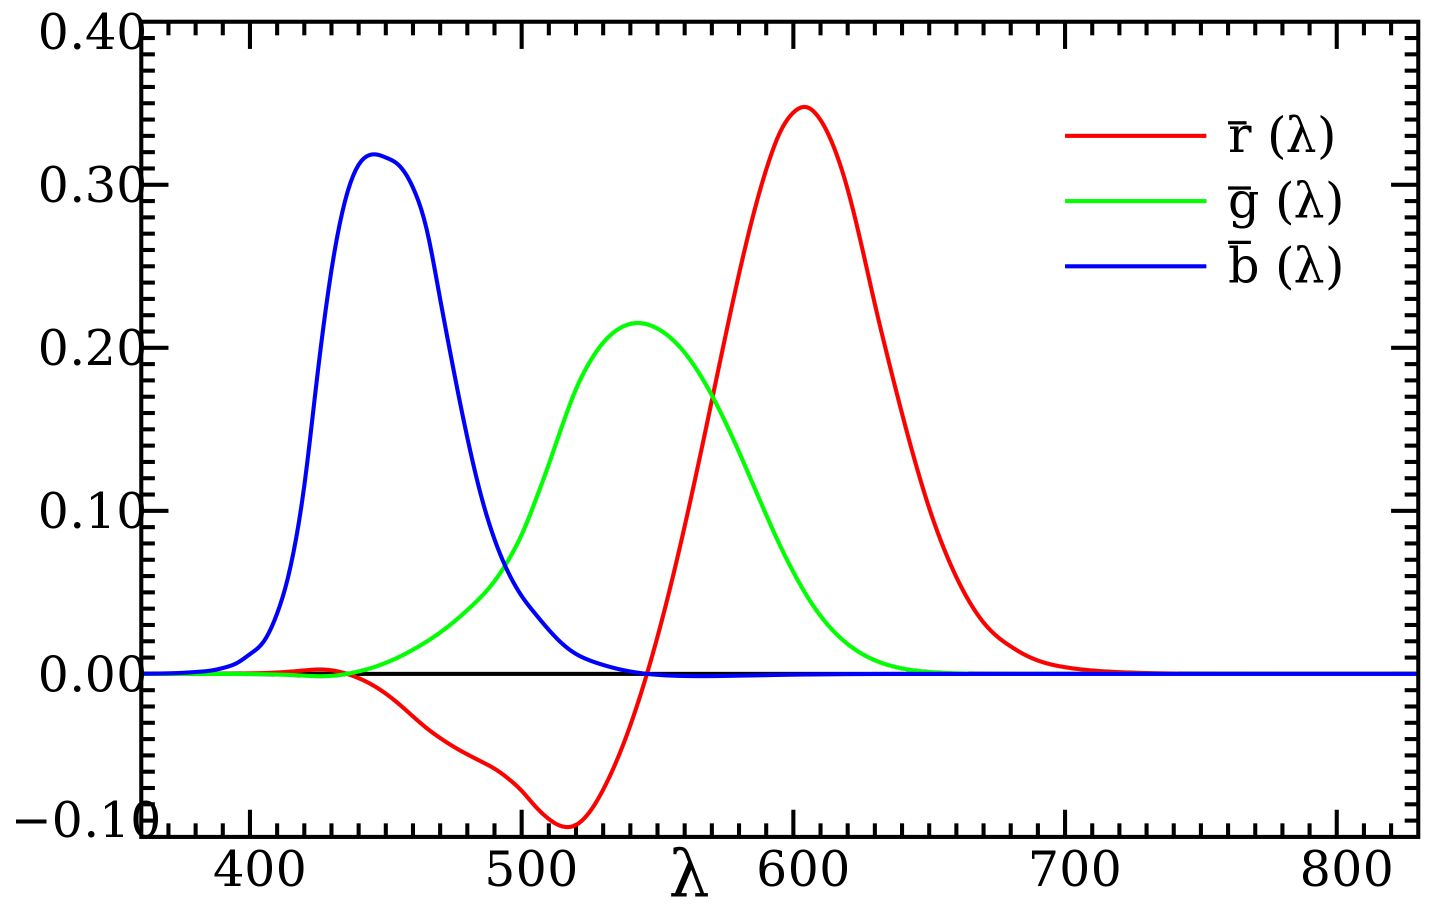
\includegraphics[scale=0.2]{color.jpg}
  \caption{光谱三刺激值}
  \label{f:光谱三刺激值}
\end{figure}

光谱三刺激值与色品坐标的对应关系如下:
\begin{equation*}
  r=\frac{\bar{r}}{\bar{r}+\bar{g}+\bar{b}}, g=\frac{\bar{g}}{\bar{r}+\bar{g}+\bar{b}}, b=\frac{\bar{b}}{\bar{r}+\bar{g}+\bar{b}}
\end{equation*}
从光谱三刺激值计算出其对应的色品坐标,最后连接各个波长的色品坐标形成光谱轨迹如图\ref{f:CIE}。

\begin{figure}[H]
  \centering
  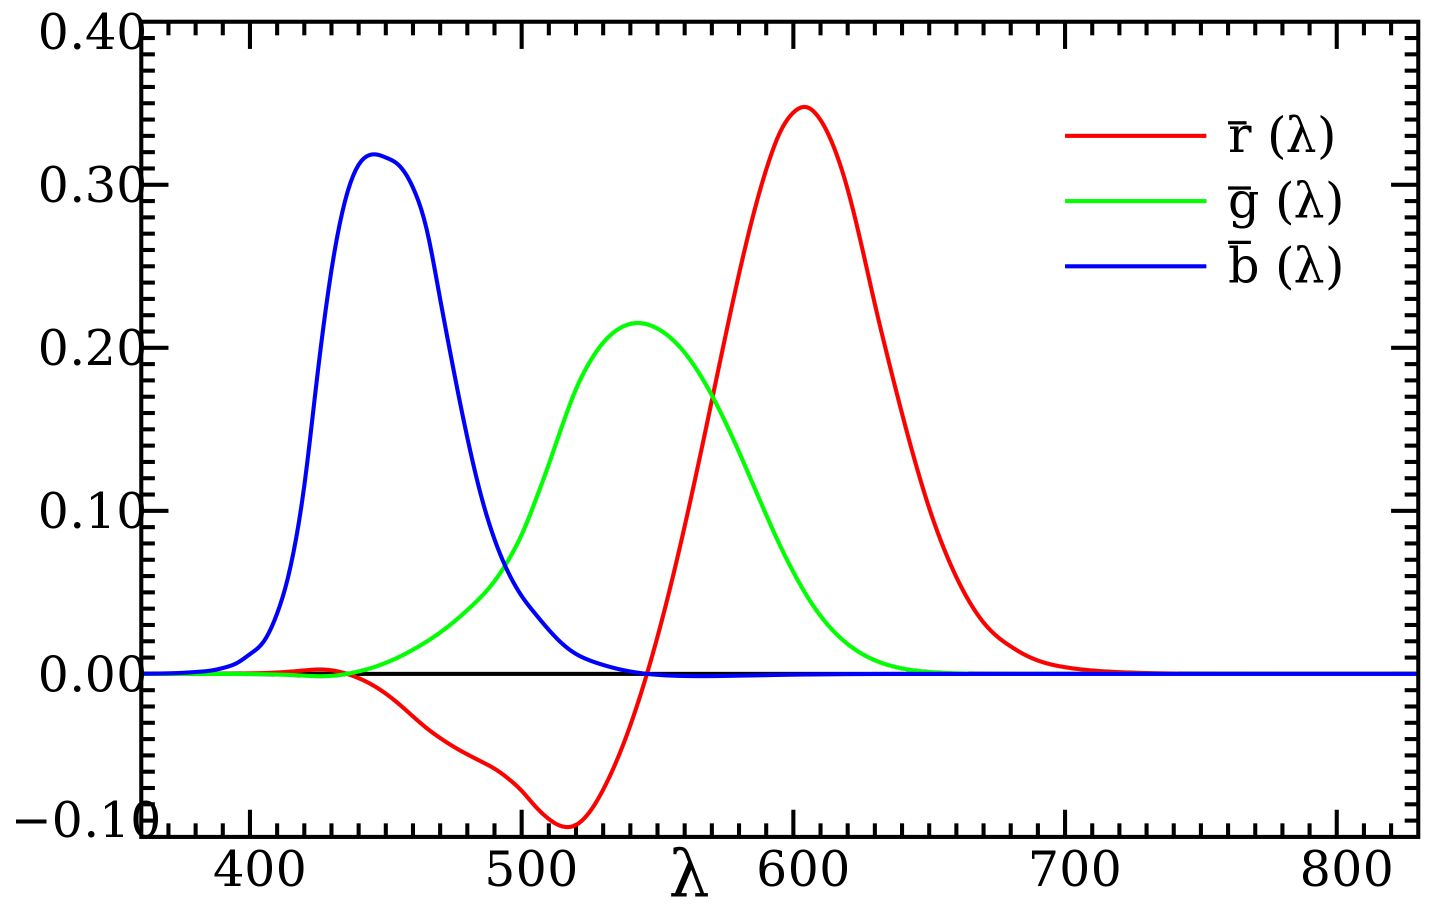
\includegraphics[scale=0.2]{color.jpg}
  \caption{CIE 1931}
  \label{f:CIE}
\end{figure}

由此,可以理解色域:色域是对一种颜色进行编码的方法,也指一个技术系统能够产生的颜色的总和。在计算机图形处理中,色域是颜色的某个完全的子集。颜色子集最常见的应用是用来精确地代表一种给定的情况。例如一个给定的色彩空间或是某个输出装置的呈色范围。



\subsubsection{从色域的角度解释为何HDR10会流行}

HDR10主要的规格包括了以下几样:
\begin{enumerate}
  \item EOTF (Electro-Optical Transfer Function):SMPTE ST 2084
  \item Color Sub-sampling:4:2:0(压缩影片)
  \item Bit Depth:10 bit
  \item 色域:ITU-R BT.2020
  \item Metadata(元数据):SMPTE ST 2086、MaxFALL、MaxCLL
\end{enumerate}

其中10 bit的影像比起以往8 bit影像可以提供更多光暗层次的数据;
BT.2020 也都比全高清时期的BT.709 色域更广阔,可以显示更多色彩。
HDR10采用的BT.2020 色域比起以往HDTV 时期的BT.709 色域广阔很多,HDTV的8 bit色深可以显示1千6百万种色彩,
如果到了10 bit的话就可以显示高达10亿种颜色。



\subsubsection{简述相加混色模型和相减混色模型的区别和联系}

\begin{itemize}
  \item 相加混色模型
\end{itemize}

相加混色,就是我们常说的RGB模式,适用于显示器等发光体的颜色显示。以黑色介质为基础,通过光源三原色不同比例的亮度叠加,来获得各种不同的颜色。

\begin{itemize}
  \item 相减混色模型
\end{itemize}

即CMY色彩模式是基于固有色光吸收/反射原理定义,适用于各种印刷媒介,以白色介质为基础,通过印刷三原色(青、品红、黄)不同比例的油墨混合,吸收原始色光中的对应波长,从而获得各种不同的颜色的反射效果,也就是所谓的相减色。例如:黄色颜料是从入射白光中吸收蓝光而反射红光和绿光所致。

\begin{itemize}
  \item 联系
\end{itemize}

相加混色模型一般运用于计算机制作出的成果想要打印的时候就需要进行不同色彩之间的转换成相减混合模型
才能印刷出人眼看到的样子。



\subsubsection{D-Sub接口某根线接触不良,屏幕泛品红色,请依据色彩空间的知识推测是哪根信号线接触不良}

品红色是介于红色和蓝色之间的颜色。
故,应该是绿色(GREEN)信号线接触不良。



% ------------------------subsection----------------------------------

\subsection{数码相机技术}

\subsubsection{分析2000年左右数码相机分辨率达到200万像素后迅速取代传统相机的原因}

200万像素已经基本上达到1080p的分辨率从分辨率角度已经能与传统相机分不出太大差距;
数码相机焦距与变焦,景深/光圈,感光度,测光、曝光与曝光补偿,白平衡,自动对焦
等功能集成使得使用者能很方便的拍照调试,降低学习成本,因此也促进了迅速取代传统相机。


\subsubsection{试对比智能手机上所用的RGBY、RYYB、QBC传感器和单反数码相机中的彩色合成原理}

\begin{itemize}
  \item RGBW传感器
\end{itemize}

红蓝绿三色滤色,每一个都会过滤掉部分光线,这就降低了亮度,因为光线
损失的比较多。而加入一个白色滤色片,白色是不会过滤光线,投过滤色片
照射到CMOS上的光线就比较多,这就增加了亮度。而亮度增加,低光环境
下的噪点就减少了,这就是华为宣称的提升照片32\%的亮度(高对比度),
低光环境下降低78\%的彩色噪点。

代价:采集色彩信息的CMOS面积下降了1/4

\begin{itemize}
  \item RYYB传感器
\end{itemize}

将传统RGBG拜耳滤镜换成了“RYYB”滤镜,将2个绿色像素(G)用黄色像
素(Y)替代。代表机型为:华为 P30、P40、Mate 40 Pro+等。和RGGB相比
,RYYB可以减轻前者在滤色过程中所带来的光之强度折损,可以让进光量
提升高达40\%。以华为P30 Pro为例,该产品的ISO高达409600,是iPhone Xs
Max的64倍!从而只需一丝亮光就能记录下纯黑环境下的颜色细节。

RYYB提升了进光量,但变相增加了红色的进光量,从而提升了弱光环境下
的表现。由于黄色像素较多,偏色问题将难以避免,同时绿色像素的缺失也
会影响饱和度。需要一套更加强大的硬件ISP和更为成熟的成像算法支持。

\begin{itemize}
  \item QBC
\end{itemize}

是quad bayer
coding的缩写。这种sensor的设计是:每个像素是有四个子像素组成,他们公用一个color filter。在非HDR模式下,四个像素合并成一个输出值,与当年Nokia 用的4100万像素出8百万像素的照片的所谓超采样是一个原理,具有降噪,增加动态范围的好处。在HDR模式时,会把四个像素分成两组,对角线方向的分到同一组,135度的那组曝光要短于45度的那组,然后再scale+combine,这样就生成完全pixel位置的HDR图像。

\begin{itemize}
  \item 单反数码相机
\end{itemize}

Sensor3彩色数字相机需要3个单色sensor获得彩色图
像的R,G,B分量,成本较高。单CCD获得彩色图像
的方法是在 CCD表面覆盖1个只含红、绿、蓝3色的马
赛克滤镜,对其输出信号通过一定的处理算法实现。
这个设计理念1976年最初由拜尔提出,所以这种滤镜
也被称作拜尔模板 (bayer pattern)。

由于每个像素只感知一种颜色(一种色谱),一个
彩色图像感知器的整体感知度比单色(全色)感知器
的感知度要低,实际中一般要低到3倍。所以,单色感
知器在光线不佳的情况下表现要好得多。


\subsubsection{请从滤波器角度分析镜头参数MTF(Modulation Transfer Function)的意义}

MTF图表描绘镜头从中心到边缘的反差对比度。
\begin{itemize}
  \item X轴(水平轴)显示从影像中心到边缘的距离。因此“$\pm 0$”代表镜头中心,不同的数值代表着朝向镜头边缘方向的距离,以毫米为单位。
  \item 在Y轴(垂直轴)上,最大值是1,表示光线百分之百完全通过镜头。
\end{itemize}

MTF结合了分辨率和对比度两种指标,表示了成像系统将分辨率转换为对比度的能力。
随着图像分辨率的升高,对比度会下降,(1mm的距离内线对更多,因此成像系统造成的模糊带来的影响也更严重,对比度会更差),
MTF表示了成像系统在分辨率升高的情况下保证对比度的能力。


\subsubsection{请从人的视觉认知特性角度解释拜尔模板 (bayer pattern)的设计}

Bayer pattern说的是COLOR FILTER的结构,分为两种:STD Bayer pattern 与Pair pattern,其中STD Bayer pattern的结构是BG/GR的,而Pair Pattern顾名思义是指BGBG/GRGR的结构,即以四行为一个单位,前两行是BG的结构,后两行是GR的结构
Bayer格式是相机内部的原始图片, 一般后缀名为.raw。很多软件都可以查看, 比如PS。我们相机拍照下来存储在存储卡上的.jpeg或其它格式的图片, 都是从.raw格式转化过来的。bayer色彩滤波阵列,由一半的G,1/4的R,1/4的B组成。

根据人眼对彩色的响应带宽不高的大面积着色特点,每个像素没有必要同时输出3种颜色。因此,数据采样时,

奇数扫描行的第1,2,3,4,…象素分别采样和输出R,G,R,G,…数据;

偶数扫描行的第1,2,3,4,…象素分别采样和输出G,B,G,B,…数据。

在实际处理时,每个象素的R,G,B信号由象素本身输出的某一种颜色信号和相邻象素输出的其他颜色信号构成。这种采样方式在基本不降低图像质量的同时,可以将采样频率降低60%以上。

 Bayer RGB与RGB Raw的主要区别在于两者输出前经过的处理不同,Bayer RGB从ADC输出,只经过了LENS SHADING,GAMMA等模块处理而后就直接输出,而RGB Raw则经过了整个ISP模块的处理,最终是经过YUV422的数据转化而来的


\subsubsection{手机相机可以获取和高端全画幅DSLR一样的分辨率,但为何DSLR价格昂贵?}

在光线等条件都良好的情况下,顺光拍摄一些小场景手机和单反不会造成太大的差别,手机和单反最大的差距就是在景深的控制上。单反镜头的光圈可调节,虽然手机也可以通过软件模拟出光圈可调节效果,通过多摄像头带来可变焦距和人像拍摄模式等,但是在光学结构上依旧存在着差异,因此在景深效果上也是不如单反拍照的;

目前手机已经可以搭配多个不同焦段的摄像头,通过光学和数码的混合变焦方式,实现了模拟单反相机的光学变焦效果,不过在实现的原理上与一般的单反相机借助镜头实现的变焦不同,手机的混合变焦只能配合后期软件算法实现长焦虚化的效果;

单反在画质、色彩解析力、宽容度上相比于手机都是有绝对的优势。而以上的优势是基于单反在影像领域堆料的结果,因此成本造价很高。


\subsubsection{请解释为何手机上常使用对比度检测(反差式)对焦?}

因为其成本相对较低,且相比相位对焦它对光线要求不高,相比激光对焦可以不增加额外的传感器的成本。对焦的过程就是通过移动镜片来使对焦区域的图像达到最清晰的过程,所以对焦成功以后,直观的感受就是焦点的清晰度最高,而焦点以外的区域表现为相对模糊的状态。
采用反差对焦的相机,当我们对准被摄物体时,镜头模组内的马达便会驱动镜片从底部向顶部移动,在这个过程中,像素传感器将会对整个场景范围进行纵深方向上的全面检测,并持续记录对比度等反差数值。找出反差最大位置后,运动到顶部的镜片则会重新回到该位置,完成最终的对焦。
所以使用反差对焦的手机在拍照过程中,如果取景框中的物体位置、内容发生了变动,我们的肉眼就可以观察到屏幕上的内容由模糊到清晰再到模糊的过程,有一种镜片在前后推拉的直观感受。
因为反差对焦的工作方式是进行对比度检测,因此相机镜片必须要前后移动完整记录所有的图像信息,然后计算对比度最高的位置,才能最终完成对焦。所以反差对焦的一个主要缺点就是耗费的时间较长。
反差对焦类似手动调焦的过程:模糊-清晰-模糊,然后重回到清晰的焦距。

\subsubsection{解释智能手机相机OIS的原理}

通过镜头内的陀螺仪侦测到微小的移动,然后将信号传至微处理器,处理器立即计算需要补偿的位移量,然后通过补偿镜片组,根据镜头的抖动方向及位移量加以补偿;从而有效地克服因相机的振动产生的影像模糊。这种防抖技术对镜头设计制造要求比较高,而且成本也相对高一些。光学防抖功能的效果是相当明显的,一般情况下,开启该功能可以降低2-3档快门速度,使手持拍摄不会产生模糊不清的现象,对于初学者来说效果非常明显。特别在大变焦相机,效果就更为明显了;因为一般变焦越大的情况下,就算是极轻微的抖动也是非常易见的,对于长焦情况下对防抖的功能需求就更大了。


\subsubsection{名词解释}

\textbf{Ultra-wide camera}
把焦距在24mm以下的镜头叫做超广角镜头。

\textbf{Telephoto camera}
长焦镜就是让你可以看得很远的镜头,一般200mm以上的镜头便是长焦镜。









% --------------------------section------------------------------------------------

\section{多媒体数据压缩}


\subsection{无损数据压缩}


\subsubsection{名词解释:UTF-8、UTF-16、UTF-32}

\textbf{UTF-8}

使用变长字节表示字符的编号
\begin{enumerate}
	\item 对于单字节的符号,字节的第一位设为 0,后面的7位为这个符号的 Unicode码,因此对于英文字母,UTF-8 编码和 ASCII 码是相同的。
	\item 对于n字节的符号 (n>1),第一个字节的前 n 位都设为 1,第 n+1 位设为 0,后面字节的前两位一律设为 10,剩下的位用来存储字符的Unicode 码 。
\end{enumerate}

\textbf{UTF-16}

使用变长字节表示字符的编号
\begin{enumerate}
	\item 对于编号在 U+0000 到 U+FFFF 的字符,直接用两个字节表示。
	\item 编号在 U+10000 到 U+10FFFF 之间的字符,用四个字节表示。
\end{enumerate}

\textbf{UTF-32}

用4个字节存储字符的编号.

还需要考虑计算机的端模式(大端、小端).


\subsubsection{某符号的Unicode数字编号为0x4E2D,写出UTF-8编号后的16进制结果}

0x4E2D:0100 111000 101101

$\Longrightarrow$ UTF-8: 1110 0100 10 111000 10 101101

即:0xE4B8AD


\subsubsection{已知信源X: {x1, x2, x3, x4, x5, x6},各信源符号的概率依次为 P(X): {0.2, 0.19, 0.18, 0.17, 0.15, 0.1, 0.01}。求霍夫曼编码,并计算编码效率}

(我怀疑是题写错了,应该有7个x,因为给了7个概率)
\begin{equation*}
	\begin{array}{l}
		H(X) = -\sum_{i = 1}^{7} p\left(x_{i}\right) \log _{2} p\left(x_{i}\right) \\ = -\left(0.2 \times \log _{2} 0.2+0.19 \times \log _{2} 0.19+0.18 \times \log _{2} 0.18+0.17 \times \log _{2} 0.17\right. \\
		\left.+0.15 \times \log _{2} 0.15+0.1 \times \log _{2} 0.1+0.01 \times \log _{2} 0.01\right) \\ = 2.609 
		\end{array}
\end{equation*}
哈夫曼编码为:

x1: 10

x2: 11

x3: 000

x4: 001

x5: 010

x6: 0110

x7: 0111\\
平均码长:2.72
编码效率:$\frac{2.609}{2.72}\times 100\% = 95.91\%$.


\subsubsection{对一个具有符号集B= {b1, b2} = {0, 1} ,设信源产生2个符号的概率分别为P(b1)=0.2, P(b2)=0.8。对二进制数1001进行算术编码(结果用十进制数表示)}

两个子间隔:[0, 0.2)和[0.2, 1]

1001: 0.2 + 0.8*0.2 + 0.8*0.2*0.2 + 0.8*0.2*0.2*0.8 = 0.4176


\subsubsection{对信息000020330011100006001101111进行行程(游程)编码}

40 12 10 23 20 31 40 16 20 21 10 41



% --------------------------------------subsection--------------------------------
\subsection{音频数据的压缩标准}


\subsubsection{话音编译码器通常可以分成哪三种类型,并举例简述其基本原理}

\begin{itemize}
	\item 波形编译码器
\end{itemize}

不利用生成话音信号的知识产生而是产生一种重构信
号,重构信号的波形和原始话音波形尽可能一致,这
种编译码器的复杂程度低。

波形编码代表:PCM(脉冲编码调制)

\begin{itemize}
	\item 音源编译码器
\end{itemize}

通过话音波形的信号中提取生成话音的参数,使用
这些参数通过话音生成模型重构出话音。在模型中声
道被等效成一个随时间变化的滤波器,叫时变滤波器,
激励函数是由白噪声,无声话音段激励或者由有声话
音段激励。传送的是解码器的信息就是滤波器的规格、
发声或不发声的标志和有声话音的音节周期,每
10~20ms更换一次。

数据率2.4bps,产生的语音质量很低,可以听懂而
已。增加数据率对于话音质量没有用,因为这是由模
型限制的,但保密性好。

\begin{itemize}
	\item 混合编译码器
\end{itemize}

混合编译码的想法是企图填补波形编译码和音源编
译码之间的间隔。波形编译码器虽然可提供高话音的
质量,但数据率低于16 kb/s的情况下,在技术上还没
有解决音质的问题;声码器的数据率虽然可降到2.4 
kb/s甚至更低,但它的音质根本不能与自然话音相提
并论。

为了得到音质高而数据率又低的编译码器,历史上
出现过很多形式的混合编译码器,但最成功并且普遍
使用的编译码器是时域合成-分析(analysis-by-synthesis,
AbS)编译码器。


\subsubsection{名词解释:听阈,痛阈,频域掩蔽,时域掩蔽}

\textbf{听阈}
刚能引起人耳听觉反应的最小声音刺激量,称为听阈。

\textbf{痛阈}
将各频率的听阈以线段连接,形成听阈曲线。若继续增加声音刺激强度刚能引起人耳不适或疼痛的最小刺激量,称为痛阈。

\textbf{频域掩蔽}
同时发出的频率接近的两个纯音,声强
低的纯音会被声强高的纯音淹没

\textbf{时域掩蔽}
在时间上相邻的声音之间也有掩蔽现象,
称为时域掩蔽。产生的主要原因是人的大脑处理信息
需要花费一定的时间。


\subsubsection{MPEG-1的层1、层2、层3编码分别使用了听觉系统的什么特性?}

\begin{itemize}
	\item 层1
\end{itemize}

频带相等的子带,使用频域掩蔽特性, 每个子带用6bit量
化。

\begin{itemize}
	\item 层2
\end{itemize}

频带相等的子带,除了使用频域掩蔽特性之外还利用了
时间掩蔽特性,低频段的子带用4比特,中频段的子带用
3比特,高频段的子带用2比特。

\begin{itemize}
	\item 层3
\end{itemize}

层3使用比较好的临界频带滤波器,把声音频带分成非等
带宽的子带,除了使用频域掩蔽特性和时间掩蔽特性之
外,还考虑了立体声数据的冗余,并且使用了霍夫曼
(Huffman)编码器。还使用了MDCT (modified discrete 
cosine transform) 把子带的输出在频域里进一步细分以达
到更高的频域分辨率。



% -----------------------------------subsection------------------------------


\subsection{图像数据的压缩标准}

\subsubsection{基于DCT变换的JPEG压缩编码算法的主要计算步骤有哪些?请给出编码框图,并说明此过程中哪些是有损的,哪些是无损的}

步骤:
\begin{enumerate}
	\item 正向离散余弦变换(FDCT)
	\item 量化(quantization)
	\item Z字形编码(zigzag scan) 
	\item 使用DPCM对直流系数(DC)进行编码
	\item 使用RLE对交流系数(AC)进行编码
	\item 熵编码(entropy coding)
\end{enumerate}
\begin{figure}[H]
	\centering
	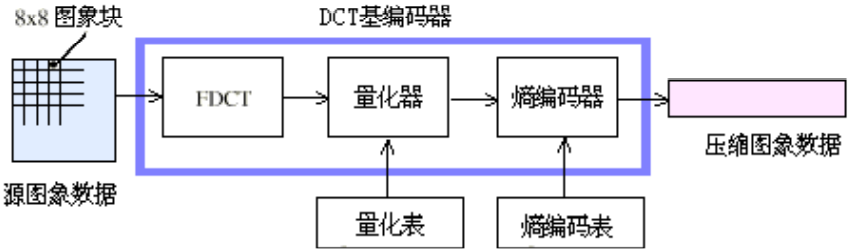
\includegraphics[scale=0.375]{dct.png}
	\caption{编码框图}
	\label{f:编码框图}
\end{figure}

但做离散余弦变换也会这一些高频成分予以抛弃,从而降低需要传输的数据量,是有损的;

量化是有损的,量化是图像质量下降的最主要原因;

ZIGZAG无损;

三步编码都有消除冗余的作用,也是有损的。



\subsubsection{JPEG利用了图像的哪几类冗余?}

第一种是编码冗余度。例如,DCT变换,哈夫曼编码,
是消除编码冗余度。

第二种是象素间冗余度。例如,直流系数用差分编码就
是消除相邻子图象间的灰度(或亮度)冗余度。

第三种是心理视觉冗余度。例如,用量化过程,就是利
用人眼对各种空间频率,包括亮度、色度、纵、横方向
的高频、低频的敏感程度不同,从而降低和消除一部分
数据,达到数据压缩的目的,或降低传输位率,同时又
不损害心理视觉对图象的主观评价。这就是充分利用心
理视觉冗余度对图象数据进行压缩。



\subsubsection{为什么JPEG使用DCT而不是DFT?}

DCT相比DFT有更好的能量聚集效果。

在扩展时,DCT采用的是对称的形式,DFT中扩展序列时,是直接采用平移方式引入了不连续的区间,而DCT采用对称形式,消除了这一人为的不连续,而通常高频信号隐藏在这人造的不连续中。

而且DFT有两种冗余:
\begin{itemize}
	\item 在有限长度实序列的DFT结果中有一半的数据是冗余的;
	\item 另外由于复数需要表示实部虚部,那么一个复数需要占用两个数据空间。
\end{itemize}
DCT的变换结果只有实数部分,没有复数部分。



------------------------subsection------------------------------
\subsection{视频数据的压缩标准}


\subsubsection{什么是视频编码中的运动补偿技术?}

运动补偿是通过先前的局部图像来预测、补偿当前的局部图像。

运动补偿是一种描述相邻帧(相邻在这里表示在编码关系上相邻,在播放顺序上两帧未必相邻)差别的方法,具体来说是描述前面一帧的每个小块怎样移动到当前帧中的某个位置去。这种方法经常被视频压缩/视频编解码器用来减少视频序列中的空域冗余。它也可以用来进行去交织(deinterlacing)与以及运动插值(motion interpolation)的操作。


\subsubsection{请画出H.264的编码框图}

\begin{figure}[H]
	\centering
	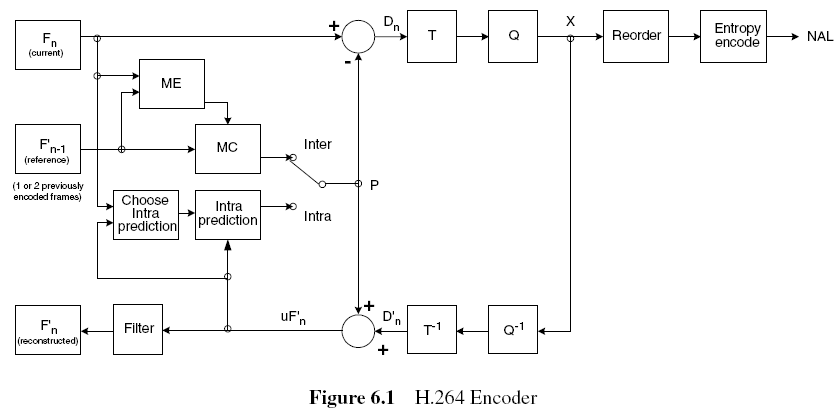
\includegraphics[scale=0.6]{h264_enc.png}
	\caption{编码框图}
	\label{f:编码框图}
\end{figure}
\begin{figure}[H]
	\centering
	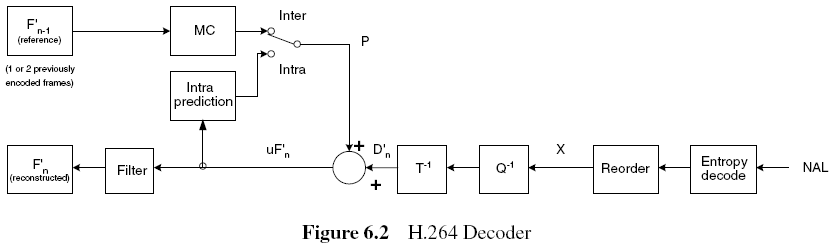
\includegraphics[scale=0.6]{h264_dec.png}
	\caption{解码框图}
	\label{f:解码框图}
\end{figure}


\subsubsection{简述Golomb-Rice编码的基本原理,并分析在什么情形下该编码能实现高的压缩比}

Golomb编码是一种基于游程编码(run-length encoding,RLE)的无损的数据编码方式。

Golomb编码是一种分组编码,需要一个正整数参数m,然后以m为单位对待编码的数字进行分组。
对于任一待编码的非负正整数N,Golomb编码将其分为两个部分:所在组的编号GroupID以及分组后余下的部分,GroupID实际是待编码数字N和参数m的商,余下的部分则是其商的余数,具体计算如下:

$$ q=N/mr=N\%mq=N/mr=N\%m $$ 
对于得到的组号q使用一元编码(Unary code),余下部分r则使用固定长度的二进制编码(binary encoding)。

设待编码的非负整数为N,Golomb-Rice编码流程如下:
\begin{enumerate}
	\item 初始化正整数参数m
	\item 取得组号q以及余下部分r,计算公式为:q=N/m,r=N\%mq=N/m,r=N\%m
	\item 使用一元编码的方式编码q
	\item 使用二进制的方式编码r,r所使用位数(Golomb-Rice编码要求参数m是2的次幂)取r的二进制表示的低log2(m)log2⁡(m)位,作为r的码字。
\end{enumerate}

\begin{itemize}
	\item 高的压缩比的情况:
\end{itemize}
当待压缩的数据符合几何分布(Geometric Distribution)时,Golomb编码取得最优效果。







% --------------------------section------------------------------------------------


\section{多媒体数据的数字存储}

\subsection{关于CD的黄皮书和红皮书存在哪些重要区别?}

\begin{itemize}
	\item 红皮书
\end{itemize}

1982年,Philips和Sony把用“1”和“0”表示的声音
信号记录到以塑料为基片的金属圆盘上。由于这种塑
料金属圆盘很小巧,所以用了英文Compact Disc来命
名。这种盘又称为数字激光唱盘(Compact Disc-Digital 
Audio,CD-DA)盘。

\begin{itemize}
	\item 黄皮书
\end{itemize}

CD-ROM 存放数字化的文、图、声、象等,1985。
但从CD-DA过渡到CD-ROM有两个重要问题需要
解决:1. 计算机如何寻找盘上的数据。2. 要求它的错
误率($10^{-12}$)远远小于声音数据的错误率($10^{-9}$),而
现成的CD-DA技术不能满足这一要求,因此还要采
用错误校正技术。于是就开发了“黄皮书(Yellow)
标准”。

CD-DA 存放数字化的音乐节目; CD-ROM 存放数字化的文、图、声、象等.


\subsection{简述 CD-DA、HDCD、SACD 的区别}

\begin{itemize}
	\item CD-DA
\end{itemize}

CD-DA又叫激光数字唱盘,用来存储数字音频信息,如音乐歌曲等。早期,Philips公司、SONY公司希望用CD来保存数字高保真音乐,为此制定的标准称为Compact Disc-Digital Audio标准,简称CD-DA标准(CD-Audio Book)。符合这个标准的光盘都标有“Digital Audio”的标识。正式标准定义在1982年发布的红皮书(Red Book)中,包括定义了CD的尺寸、物理特性、编码方式、错误校正等。

\begin{itemize}
	\item HDCD
\end{itemize}

为改善现有CD记录格式的缺陷,使之既能高度兼容而在音质上又能有所突破,美国Pacific Microsonics公司推出了具有专利保护的HDCD录播新技术,它的英文全称是High Definition Compatible Digital,译为高解析度的CD。用HDCD方式编码制造的激光唱片与普通CD具有高度的兼容性,用在普通的激光唱机上播放,已可领略到HDCD编码录音技术的优越性,如用带有HDCD解码功能的CD唱机播放,则可充分欣赏到全部释放的HDCD信息所特有的魅力:音质清晰细腻、动态范围广阔、信噪比极高,音色更为自然逼真。

HDCD的编码与制造

针对传统CD录音格式的局限与不足,PM公司的两位HDCD创始人,Keith O·Johnson录音师和Michael W.pflaumer计算机专家在多年音响制作中,查找并证实了对CD音质影响的几个关键因素,并提出切实可行的解决方案。

HDCD技术是在前期录音制作中即重视所录制信号的完整和精确性,采用高于常规两倍的取样频率88.1kHz对模拟信号进行采样,以最大限度地展宽高频响应,减少缺损性失真,高的采样率也为HDCD编码运算留足了空间。

用24bit量化其取样值为1677216个,它比16bit系统高出256倍,采用高位元处理技术可以提高处理精度,降低量化误差,增加动态范围至120dB。

在模拟至数字信号转换过程中,HDCD技术十分重视转换精度,尽量减少串音和处理的稳定性,其能够达到的指标为转换精度百万分之一,失真分量<-120dBfs。

这个高精度、宽频带的数字信号构成HDCD编码制造的基础,其数据信息量十分庞大。用常规CD PCM编码格式无法将其容纳。如要在普通CD机上兼容播放,需经特殊运算编码方可。

用高采样和高比特技术进行CD的录音制作已被普遍认可和广泛采用,但提醒一点是目前市场上所能见到的20、24bit CD激光唱盘其实质应是录音过程中采用的比特数,由于CD“红皮书”所制定的44.1kHz/16bit标准格式制约,这些高信息量的母带在灌制CD唱片时,均经过重新运算,编码制成16bit的CD唱片。因此,我们现在CD唱机所能解读出来的规格仍然是16bit/44.1kHz,由于各唱片公司在转化过程所采用手法不同,我们现在能听到的不同版本的CD音质也的确各有千秋,但有一点可以肯定:高比特高取样技术制作的CD音质远胜16bit/44.1kHz录音格式制作的 CD。

\begin{itemize}
	\item SACD
\end{itemize}

SACD全称叫Super Audio CD,是超级音频光盘系统,它是由索尼和飞利浦公司合作开发的一款具有全面取代CD音源实力的最新格式的数码系统。SACD采用DSD数字录音技术,它的频率范围和动态范围均优于CD。SACD是一种新型的光盘,它不是CD格式,而类似DVD光盘,播放时需使用SACD专用的播放设备。

SACD 光盘结构大致与DVD相似,播放面有单面和双面,信息层有单层和双层。目前市场上的SACD光盘较多采用单面双层结构,一层是0.6mm基片上储存 16bits传统CD格式的信号,可与CD兼容,另一层是0.6mm基片高密度的半透明层,储存SACD格式的信号,再将两片基片像DVD盘片那样粘合而成。这种光盘可以在普通CD播放机上播放,也可以在SACD播放机上播放,当然,两者的音质是有差别的。
SACD的技术指标远优于CD,而与DVD-Audio相似。
SACD的核心技术是DSD (Direct Stream Digital 直接数据流),它与CD、DVD-Audio的多bit录制原理有根本的区别。


\subsection{简述在 VCD、DVD、EVD、HD-DVD 和 BlueDVD 系统中的信源编码和信道编码}

% Table generated by Excel2LaTeX from sheet 'Sheet1'
\begin{table}[H]
	\centering
	% \caption{Add caption}
		\begin{tabular}{|l|p{16.2em}|l|}
		\toprule
			& \multicolumn{1}{l|}{音频} & 视频 \\
		\midrule
		VCD   & \multicolumn{1}{l|}{MPEG1 Audio} & MPEG1 \\
		\midrule
		DVD   & \multicolumn{1}{l|}{Dolby AC-3 DTS(D9)} & MPEG2 MP@ML \\
		\midrule
		EVD   & \multicolumn{1}{l|}{EAC} & MPEG2 MP@HL \\
		\midrule
		HD-DVD & Dolby Digital Plus\newline{}DTS++Lossy & \multicolumn{1}{l|}{\multirow{2}[4]{*}{MPEG-2, ~~\newline MPEG-4 AVC, ~\newline VC-1}} \\
	\cmidrule{1-2}    BD    & DTS 5.1 Dolby Digital 5.1\newline{}7.1-channel 96/24 PCM &  \\
		\bottomrule
		\end{tabular}%
	% \label{tab:addlabel}%
\end{table}%







% --------------------------section------------------------------------------------

\section{多媒体信息分析与理解}


\subsection{简述常见链接分析算法及其基本思想}

\begin{itemize}
	\item HITS (Hypertext Induced Topic Selection)
\end{itemize}

描述了权威网页和中心网页之间的一种依赖关系:一个
好的中心网页应该指向很多好的权威性网页,而一个好
的权威性网页应该被很多好的中心性网页所指向。

\textbf{基本思想:}

HITS定义了两个参数来描述网页
\begin{enumerate}
	\item a(v) – authority,权威度描述有多少重要的网页指向它
	\item h(v) – hubness,导航性描述它指向多少重要的网页
\end{enumerate}
\begin{figure}[H]
	\centering
	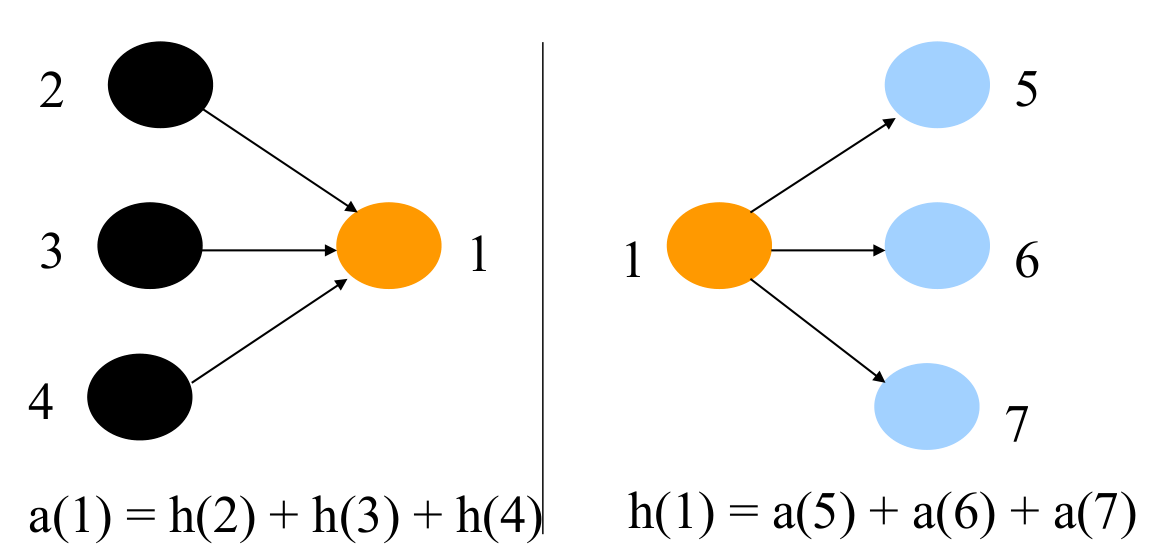
\includegraphics[scale=0.2]{hits.png}
	\caption{HITS}
	\label{f:hits}
\end{figure}

\begin{itemize}
	\item PageRank
\end{itemize}

利用网络自身的超链接结构给所有的网页确定一个重要
性的等级数,当从网页A链接到网页B时,就认为“网页
A投了网页B一票”,增加了网页B的重要性。最后根据
网页的得票数评定其重要性,以此来帮助实现排序算法
的优化。

\textbf{基本思想:}

Page et al (1998)提出网页的重要性取决于
指向它的链接
\begin{figure}[H]
	\centering
	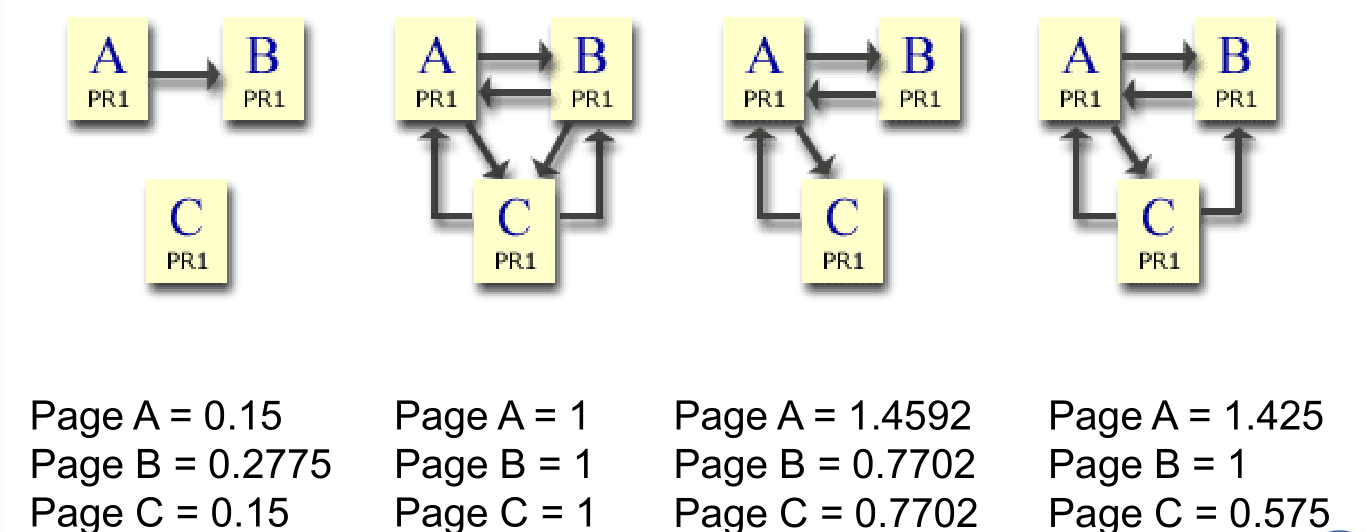
\includegraphics[scale=0.225]{pagerank.png}
	\caption{PageRank}
	\label{f:pagerank}
\end{figure}



\subsection{基于内容的图像检索常用的相似度度量方法有哪些?}

\begin{enumerate}
	\item SSIM算法—结构相似性:
	
	SSIM(structural similarity)是一种用来衡量图片相似度的指标,也可用来判断图片压缩后的质量。SSIM取值范围[0, 1],值越大,表示图像失真越小。
基本原理:
SSIM由亮度对比、对比度对比、结构对比三部分组成。亮度比较函数l(x,y)是μx和μy的函数。
然后,对比度比较c(x,y)是σx和σy的比较。
这三个组成部分相对独立。 例如,亮度和/或对比度的变化不会影响图像的结构。
C1、C2、C3为常数,避免分母接近于0时造成的不稳定性。
SSIM函数S具有对称性、有界性(不超过1)和最大值唯一性(当且仅当x=y时,S=1,表示两幅图一样)。
	\item Siamese network:
	
	Siamese Network 是一种神经网络的框架,而不是具体的某种网络,用于评估两个输入样本的相似度。
	两个网络分别接受输入,共享权重,然后计算两个输出向量之间的距离或者相似度,以此来判别原输入的相似性。例如判别两张脸是否为同一个人的,两个签名是否为同一个人所作。当然,siamese network不仅只适用这种二分类问题,在目标跟踪领域也被广泛的应用如siamMask。
图中上下两个network,都由CNN构成,两个模型的参数值完全相同。不同于传统CNN的地方,是Siamese网络并不直接输出类别,而是输出一组一维向量。
若输入的两张图像为同一个人,则上下两个模型输出的一维向量欧氏距离较小
若输入的两张图像不是同一个人,则上下两个模型输出的一维向量欧氏距离较大
所以通过对上下两个模型输出的向量做欧氏距离计算,就能得到输入两幅图像的相似度
	\item 均值Hash算法:
	
	Hash算法进行图片相似度识别的本质,就是将图片进行Hash转化,生成一组二进制数字,然后通过比较不同图片的Hash值距离找出相似图片。
	\begin{enumerate}
		\item 缩小尺寸。这样做会去除图片的细节,只保留结构、明暗等基本信息,目的是统一图片大小,保证后续图片都有相同长度的哈希值,方便距离计算。网上看到的案例基本都将尺寸缩小为8*8,64个像素点,暂时不清楚缩小为这个尺寸的原因,但如果觉得损失的信息太多,可以将尺寸适当调大,当然像素点多了后续计算就会稍慢一些。
		\item 灰度化处理。将图片全部转换为统一的灰度图。
		\item 计算像素均值。计算像素的灰度平均值(此处均值出现)
		\item 哈希值计算。将每个像素的灰度,与平均值进行比较。大于或等于平均值,记为1,小于平均值,记为0,由此生成二进制数组。
		\item 图片配对,计算汉明距离。距离越近,越相似。当图片缩小为8 * 8时,通常认为汉明距离小于10的一组图片为相似图片。PS:(汉明距离:它就是将一个字符串变换成另外一个字符串所需要替换的字符个数。)
	\end{enumerate}
	优点:速度快;
缺点:精确度较差,对均值敏感
	\item 差异哈希算法
	\item 感知哈希算法
	\item cosin相似度
	\item 皮尔逊相关系数
\end{enumerate}



\subsection{什么是语义鸿沟?}

相似的视觉特征 (颜色、纹理、形状等)可能表达完
全不同的语义。

语义鸿沟:底层视觉特征和高层语义概念间的差距。
特征相似的图像可能完全不相关,
低层特征和图像意义没有必然联系。





% --------------------------section------------------------------------------------

\section{实时多媒体通信}


\subsection{QoS的评价参数有哪些,简述它们的基本概念}

QoS(Quality of Service)参数:
\begin{itemize}
	\item 可用带宽
	
	网络的两个节点之间特定业务流的平均速率
	\item 时延
	
	数据包在网络的两个节点之间传送的平均往返时间
	\item 丢包率
	
	在网络传输过程中丢失报文的百分比
	\item 时延抖动
	
	时延的变化
	\item 误包率
	
	网络传输中报文出现错误的百分比
\end{itemize}



\subsection{RTSP、MMS、RTMP、HLS等协议完成的主要功能是什么?}

\begin{itemize}
	\item RTSP (Real Time Streaming Protocol)
\end{itemize}

由RealNetworks和Netscape提出,RTSP通过RTP传送
的是多媒体数据。HTTP只能由客户机发出请求;RTSP客户机和服务器都可以
发出请求,即RTSP可以是双向的。

\begin{itemize}
	\item MMS (Microsoft Media Server Protocol)
\end{itemize}

MMS是微软定义的用来访问并流式接收 Windows
Media 服务器中*.asf 文件的一种协议

\begin{itemize}
	\item RTMP(Real Time Messaging Protocol)
\end{itemize}

RTMP(Real Time Messaging Protocol)实时消息传送
协议是Adobe 为Flash播放器和服务器之间音频、视频
和数据传输 开发的开放协议。

\begin{itemize}
	\item HLS (HTTP Live Streaming)
\end{itemize}

HLS点播,基本上就是常见的分段HTTP点播,不同在于,它
的分段非常小。要实现HLS点播,重点在于对媒体文件分段,
目前有不少开源工具可以使用。

相对于常见的流媒体直播协议,例如RTMP协议、RTSP协议、
MMS协议等,HLS直播最大的不同在于,直播客户端获取到的,
并不是一个完整的数据流。HLS协议在服务器端将直播数据流
存储为连续的、很短时长的媒体文件(MPEG-TS格式),而客
户端则不断的下载并播放这些小文件,因为服务器端总是会将
最新的直播数据生成新的小文件,这样客户端只要不停的按顺
序播放从服务器获取到的文件,就实现了直播。

可以认为,HLS是以点播的技术方式来实现直播。由于数据
通过HTTP协议传输,所以完全不用考虑防火墙或者代理的问
题,而且分段文件的时长很短,客户端可以很快的选择和切换
码率,以适应不同带宽条件下的播放。不过HLS的这种技术特
点,决定了它的延迟一般总是会高于普通的流媒体直播协议。




\subsection{多媒体会议系统的基本组成与一般结构是什么?}

基本组成:
显示系统,音频扬声器系统,矩阵开关系统和数字,中间控制系统,环境控制系统等组成。

子系统结构:
\begin{itemize}
	\item 数字会议系统(发言、表决、同传等);
	\item 会议场扩音系统(会议扩音、多动能扩音);
	\item 灯光舞台系统(环境灯光、摄像灯光、舞台灯光、舞台机械);
	\item 显示系统(投影、液晶、等离子、LED,拼接、边缘融合等);
	\item 摄录编播系统(监控摄像、会议摄像、广播摄像,录像及处理);
	\item 信号处理系统(信号的分配、切换、传输、转化,图像处理等);
	\item 集中控制系统(AV中心智能化联动控制系统);
	\item 会议支撑系统(机房、网络、远程会议、视频会议等);
	\item 数字音视专业布线系统。
\end{itemize}















% \bibliographystyle{gbt7714-numerical}
% % \bibliographystyle{7714-author-year}
% \bibliographystyle{ieeetr}
% \bibliography{bibl}

\end{document}